
%   i.) Describe all the steps of a Deep Learning FL system
%
%

%how do FL systems work in general?
%
Feature location systems retrieve a ranked list of program elements (e.g.
methods, classes) for a developer query. In the {\em training} phase, feature
location systems commonly construct a model of the software, at the granularity
of program elements, based on the natural language embedded in identifiers and
comments. In the {\em retrieval} phase, given a natural language query, feature
location systems use the model to retrieve all of the relevant program elements
with high similarity to the query.

\subsection{Feature Location Workflow}

%how does a deep learning system differ
%
A feature location system based on deep learning, during its training phase,
creates a contextual representation of the natural language terms embedded in
the source code. This contextual representation includes influence from terms
preceding and following each term, relative to their distance from that term.
More intuitively, such models incorporate mutual influence between terms in the
same method, while terms that are closer in distance (e.g. occur the same
statement) influence each other more strongly.


\begin{figure}[tb]
\centering
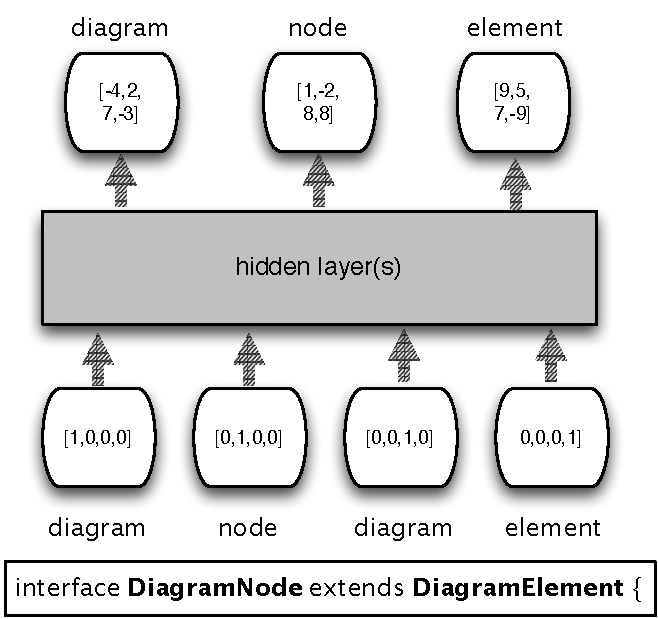
\includegraphics[width=.9\columnwidth]{figures/neuralnet.pdf}
\caption{A deep learning neural network encodes source code identifiers, in the
order they appear in the source code, in its input layer. Using a deep
structure of hidden layers, each term and its context receives a semantic
vector representation. The output layer consists of vector for each term in
the corpus; the vector feature size is arbitrary and does not need to relate to
the number of terms in the corpus.}
\label{fig:neuralnet}
\end{figure}


%what is deep learning
Deep learning is based on a multi-stage neural network, consisting of several
hidden layers in addition to single input and output layers.  The input layer
consists of an ordered sequences of identifiers extracted from the code. The
multiple hidden layers serve to capture the context for each encountered term,
representing the complex patterns of term contexts occurring in the corpus. The
output layer consists of a vector for each term, which has been shown to carry
semantic meaning. An example of this architecture for a single line of code is
shown in Figure~\ref{fig:neuralnet}. Recent advances in this area have stemmed
from the use of novel neural network architectures, including recurrent neural
networks that connect the hidden layers back to the input layer, among other
strategies. The systems are trained using backpropagation and gradient descent,
techniques common to many neural network based models.

%paragraph2vec
An extension to learning the semantic vector representation of words is the use
of an additional vector that will encode the representation of a larger body of
text, such as a paragraph or an entire document~\cite{le_distributed_2014}.
While comparing word vectors indicates semantic relations between two terms,
comparing two document vectors carries a similar semantic connotation at the
document level. For instance, the approach has been applied for determining the
sentiment (i.e. positive, negative) of reviews on a popular movie recommendation
site.

%preprocessing
A number of preprocessing steps are commonly performed before the training phase
of feature location systems.  
The steps commonly used are~\cite{Marcus-etal_2004,Marcus-Menzies_2010}: % that we use are:
\begin{itemize}
    \item {\it Splitting}: separate tokens into constituent words based on
        common coding style conventions (e.g., the use of camel case or
        underscores) and on the presence of non-letters (e.g., punctuation or
        digits)
    \item {\it Normalizing}: replace each upper case letter with the
        corresponding lower case letter
    \item {\it Filtering}: remove common words such as articles (e.g., `an' or
        `the'), programming language keywords, standard library entity names, or
        short words
\end{itemize}


%retrieval
During the retrieval state of feature location, a similarity measure (e.g.
cosine similarity) between the words in the query and words in each program
element is computed. The program elements are ranked based on this similarity
metric and presented to the developer in descending order.

If document vectors are used then a special inference process is needed to infer
a vector representation for the entire query, treated as a document in the
corpus. Following this, the vectors of the query and each program element (i.e.
method or class) can be compared to produce the final ranking.

\subsection{Semantic Similarity}


\begin{table*}[tb]
\centering
\small
\caption{Examples of semantically similar terms and their weight for a deep model trained on
the ArgoUML code base. Only terms with weight > 0.6 are included.}
\label{tab:semsim}
\begin{tabular}{|p{0.30\textwidth}|p{0.60\textwidth}|}
\hline \hline
{\em Term(s)} & {\em Semantically Similar Terms and Weight}\\ \hline \hline
association & (roles 0.75), (role 0.72), (classifier 0.72), (connection, 0.61) \\ \hline
save & (saved 0.69), (pcs 0.64), (exists 0.63), (projects 0.60), (close 0.61), (file 0.60) \\ \hline
file & (filter 0.78), (zip 0.74), (exists 0.74), (persister 0.71), (files 0.69), (directory 0.69) \\ \hline
file + save & (exists 0.77), (saved 0.74), (filter 0.73), (zip 0.72), (unable 0.67), (projects 0.67), (persister 0.67), (files 0.66), (cant 0.66), (scheme 0.65) \\ \hline
explorer + diagrams - creating & (nodes 0.71), (deletion 0.67), (perspectives 0.65), (perspective 0.60), (updated 0.60), (modified 0.60)\\
\hline \hline
\end{tabular}
\end{table*}

The result of the deep learning models described in this paper are vectors
representing each term in the corpus~\cite{mikolov_distributed_2013}. Similar
vectors can also be computed to represent an entire paragraph or
document~\cite{le_distributed_2014}. Semantic similarity is the notion that
these vectors are composable semantically, e.g., the result of the operation
{\em vec(``The Eiffel Tower'') - vec(``Paris'') + vec(``London'')} is closest to
{\em vec(``Big Ben'')}. This capability is established automatically by the
system, without any additional processing or supervised input.

In feature location, as in general information retrieval, the retrieval quality
can only be as good as the quality of the developer query. Problems such as the
dictionary mismatch problem, as well as the propensity of users to issue short
queries, have previously been observed as common difficulties in using feature
location tools in the field~\cite{haiduc_effect_2011, damevski_field_2015}.
Semantic similarity can be a useful capability in mitigating these problems, by
performing query recommendation that allows the user to extend his or her
queries with terms from the same corpus, or automatic query extension.

To illustrate this capability for source code-based corpora, we provide a set of
illustrative examples gathered on the ArgoUML v0.22 in Table~\ref{tab:semsim}.
In many cases semantic similarity provides reasonable results for similar terms,
though exceptions exist largely due to the limited appearance of certain words
in the corpus.  We anticipate that larger corpora, based on larger code bases,
or leveraging related code bases or documents, could improve the results of
semantic similarity even further.


